\documentclass{article}

\usepackage[nonatbib, final]{neurips}
\usepackage[numbers]{natbib}

\makeatletter
\renewcommand{\@noticestring}{
  \centering

}
\makeatother

\usepackage[export]{adjustbox}
\usepackage[ruled]{algorithm2e}
\usepackage[inline, shortlabels]{enumitem}
\usepackage[T1]{fontenc}
\usepackage{hyperref}
\usepackage{microtype}
\usepackage{pifont}
\usepackage{xcolor}
\usepackage{xurl}
% Figures and Tables
\usepackage{graphicx}
\usepackage{booktabs}
\usepackage{tabularray}
\usepackage{subcaption}
% Monospaced Code Blocks
\usepackage{listings}
% Math Packages
\usepackage{amsmath, amsfonts, amssymb}
\usepackage{nicefrac}

\UseTblrLibrary{booktabs}

\lstset{
  backgroundcolor=\color{white},
  basicstyle=\ttfamily\small,
  breakatwhitespace=false,
  breaklines=true,
  captionpos=b,
  columns=fullflexible,
  commentstyle=\color{gray},
  escapeinside={\%*}{*)},
  extendedchars=true,
  frame=none,
  keepspaces=true,
  keywordstyle=\color{blue},
  language=Python,
  numbers=none,
  numbersep=5pt,
  numberstyle=\color{black},
  rulecolor=\color{black},
  showspaces=false,
  showstringspaces=false,
  showtabs=false,
  stepnumber=1,
  stringstyle=\color{red},
  tabsize=4,
}

\makeatletter
\newcommand{\ssymbol}[1]{\@fnsymbol{#1}}
\newcommand{\romanNumeral}[1]{\expandafter\@slowromancap\romannumeral #1@}
\makeatother

% Custom commands for the paper
\newcommand{\oc}{\textsc{OpenCausality}}
\newcommand{\eg}{e.g.,\xspace}
\newcommand{\ie}{i.e.,\xspace}
\usepackage{xspace}


\title{\oc{}: Auditable Agentic Causal Inference \\
with DAG-Based Reasoning and LLM-Assisted Discovery}

\author{
    Chenyu Li \\
    Columbia University \\
    \href{mailto:cl4183@columbia.edu}{cl4183@columbia.edu}
}

\begin{document}

\maketitle

%% ============================================================
%% ABSTRACT
%% ============================================================
\begin{abstract}
We introduce \oc{}, an open-source platform that resolves the automation--transparency tradeoff in applied causal inference. \oc{} combines DAG-based causal reasoning with agentic estimation pipelines, where every modeling decision---from identification strategy selection to effect propagation---is logged in a hash-chained audit trail. An always-on \emph{sentinel loop} runs continuously in the background, re-validating the DAG after every change, auto-fixing schema regressions, and surfacing interactive review panels---so analysts never have to hunt for results or wonder whether the specification is still valid. The platform enforces 29 issue-detection rules that catch overclaiming, control shopping, and specification drift; a 7-guardrail propagation engine that performs unit-aware dimensional analysis across multi-edge causal paths; and a 3-stage identifiability screen that downgrades claims based on diagnostic evidence rather than statistical significance alone. A 4-agent agentic loop (DataScout, ModelSmith, Estimator, Judge) iterates between estimation, issue detection, and auto-repair under LLM guidance, while an LLM-assisted pipeline extracts causal claims from the literature and proposes DAG edges---achieving 100\% estimate precision on matched edges in our Kazakhstan bank stress-testing case study while discovering 3 edges absent from the expert-built DAG. All governance decisions---including human-in-the-loop gates and automated patch policies that explicitly prohibit p-hacking---are recorded with cryptographic integrity. \oc{} ships with 18 estimation adapters spanning econometric and ML-based methods, a data-driven causal discovery agent (PC, GES, FCI, NOTEARS), a DoWhy refutation engine for post-estimation robustness, a natural-language query interface, and 204 passing tests across 40{,}969 lines of code.
\end{abstract}

%% ============================================================
%% 1  INTRODUCTION
%% ============================================================
\section{Introduction}
\label{sec:intro}

Applied causal inference faces a fundamental tension: automation accelerates analysis but obscures the chain of decisions that produced the results. A researcher running a modern causal-ML pipeline can obtain point estimates in seconds, yet documenting \emph{why} a particular identification strategy was chosen, which controls were included, and what diagnostic checks were performed remains a manual, error-prone process. This opacity undermines reproducibility and invites specification searching~\citep{simmons2011false}.

Existing frameworks address parts of this problem. DoWhy~\citep{sharma2020dowhy} formalizes the identify-estimate-refute workflow. EconML~\citep{battocchi2022econml} provides heterogeneous treatment-effect estimators. CausalML~\citep{chen2020causalml} targets uplift modeling. However, none of these systems treats every estimation decision as an auditable event, enforces claim-level restrictions based on identification strength, or prevents automated specification searching through explicit policy enforcement.

We introduce \oc{},\footnote{Code and data: \url{https://github.com/LEE-CHENYU/OpenCausality}} an open-source platform that makes the entire causal inference workflow---from DAG construction to effect propagation to human review---both automated and transparent. Our key insight is that \emph{the audit trail is not a byproduct of estimation; it is a first-class output}. Every edge estimate, diagnostic result, issue flag, and governance decision is recorded in a hash-chained ledger that can be committed to version control and independently verified. An always-on sentinel loop runs alongside estimation, continuously validating the DAG, auto-healing schema regressions, and surfacing interactive panels---ensuring that the specification never silently degrades.

\paragraph{Contributions.} We make the following contributions:

\begin{enumerate}[leftmargin=*, itemsep=2pt]
    \item A \textbf{DAG-based causal inference platform} with 18 estimation adapters (econometric and ML-based), mode-aware effect propagation, unit-dimensional analysis across 9 unit types, and 7 guardrails that gate edge usage based on identification strength, time-series diagnostics, and issue severity (Section~\ref{sec:propagation}).

    \item A \textbf{29-rule issue detection engine} with a PatchPolicy whitelist that explicitly prohibits control shopping, sample trimming, lag searching, and outcome switching---preventing automated p-hacking while permitting safe auto-fixes (Section~\ref{sec:issues}).

    \item A \textbf{3-stage identifiability screen} (pre-design, post-design, post-estimation) backed by TSGuard, a 7-diagnostic time-series validator that caps claim levels based on evidence rather than significance, and a DoWhy refutation engine that stress-tests estimates via 4 robustness checks (Section~\ref{sec:identification}).

    \item An \textbf{LLM-assisted NL-to-DAG pipeline} that extracts causal claims from academic text, and a \textbf{data-driven causal discovery agent} (PC, GES, FCI, NOTEARS) with graph-format interoperability (NetworkX, DoWhy GML, pywhy-graphs ADMG), achieving 100\% estimate precision on matched edges while discovering novel edges absent from expert specifications (Sections~\ref{sec:llm}--\ref{sec:discovery}).

    \item A \textbf{hash-chained governance framework} with human-in-the-loop gates, structured checklists, and cryptographic audit integrity---all without database dependencies (Section~\ref{sec:governance}).

    \item An \textbf{always-on sentinel loop} that continuously validates the DAG, auto-heals schema regressions via PatchBot, and surfaces interactive panels (DAG visualization, HITL review board) without manual intervention; and a \textbf{4-agent agentic pipeline} (DataScout, ModelSmith, Estimator, Judge) with LLM-assisted DAG auto-repair (Section~\ref{sec:sentinel}).
\end{enumerate}

We evaluate \oc{} on a Kazakhstan bank stress-testing case study involving 32 nodes and 20 causal edges, comparing expert-built DAGs against both LLM-extracted and data-driven discovery DAGs, and verifying pipeline reproducibility across 204 tests (Section~\ref{sec:experiments}).

%% ============================================================
%% 2  RELATED WORK
%% ============================================================
\section{Related Work}
\label{sec:related}

\paragraph{Causal inference frameworks.}
One line of work provides programmatic interfaces for causal estimation. DoWhy~\citep{sharma2020dowhy} implements an identify-estimate-refute loop using graphical criteria, while EconML~\citep{battocchi2022econml} extends this with double/debiased ML and heterogeneous treatment-effect estimators. DoubleML~\citep{bach2022doubleml} focuses on Neyman-orthogonal score functions. CausalML~\citep{chen2020causalml} targets uplift modeling for business applications. These frameworks automate estimation but do not enforce claim-level restrictions, detect specification searching, or maintain hash-chained audit trails. \oc{} builds on their estimator building blocks while adding governance, propagation, and auditability layers.

\paragraph{Causal discovery.}
Classical algorithms---PC~\citep{spirtes2000causation}, GES~\citep{chickering2002optimal}, and NOTEARS~\citep{zheng2018dags}---learn DAG structure from observational data. causal-learn~\citep{zheng2024causallearn} and gCastle~\citep{zhang2021gcastle} provide implementations. \oc{} integrates these algorithms directly via a \texttt{DiscoveryAgent} that wraps PC, GES, FCI, and NOTEARS with lazy imports, compares discovered structures against existing DAGs, and routes proposed edges through HITL governance (Section~\ref{sec:discovery}). Our LLM-assisted pipeline (Section~\ref{sec:llm}) offers an alternative discovery path via literature extraction.

\paragraph{LLMs for causal reasoning.}
Recent work explores whether LLMs can perform causal reasoning from text. \citet{kiciman2023causal} evaluate LLMs on pairwise causal discovery benchmarks. \citet{long2023can} use LLMs to generate causal graphs from domain knowledge. Our approach differs in two ways: we extract causal claims with explicit identification strategies (not just pairwise directions), and we integrate extracted edges into a governed estimation pipeline rather than treating them as final outputs.

\paragraph{Reproducibility and auditing.}
The replication crisis~\citep{ioannidis2005why} has motivated pre-registration~\citep{nosek2018preregistration} and specification-curve analysis~\citep{simonsohn2020specification}. \oc{} operationalizes these concerns at the platform level: every decision is logged, issue rules catch post-hoc rationalization, and PatchPolicy prevents automated specification searching.

%% ============================================================
%% 3  SYSTEM ARCHITECTURE
%% ============================================================
\section{System Architecture}
\label{sec:architecture}

\oc{} is organized around five layers (Figure~\ref{fig:architecture}):

\begin{enumerate}[leftmargin=*, itemsep=1pt]
    \item \textbf{DAG Layer}: Parses YAML-specified DAGs with typed nodes (observed, latent, policy) and typed edges (causal, reaction function, bridge, identity). Validates acyclicity, unit presence, and node-source bindings.

    \item \textbf{Estimation Layer}: Dispatches edges to one of 18 adapters via a unified \texttt{EstimationRequest} $\to$ \texttt{Adapter.estimate()} $\to$ \texttt{EstimationResult} interface. Adapters span econometric methods (local projections, panel FE, IV-2SLS, DiD, RDD, regression kink, synthetic control) and ML-based methods (DoWhy backdoor/IV/frontdoor, DoubleML PLR/IRM/PLIV, EconML CATE, CausalML uplift). A config-driven registry dynamically loads adapters from YAML.

    \item \textbf{Inference Layer}: Runs 3-stage identifiability screening, TSGuard diagnostics, DoWhy refutation tests (4 robustness checks), 29-rule issue detection, and 7-guardrail effect propagation. Produces EdgeCards (YAML artifacts combining estimates, diagnostics, identification results, and literature references).

    \item \textbf{Governance Layer}: Hash-chained audit log, HITL gate with structured checklists, PatchPolicy enforcement, and notification system. No database dependency---the entire audit trail lives in append-only JSONL files that can be committed to Git.

    \item \textbf{Sentinel Layer}: An always-on background monitor that wraps the entire pipeline. After every step, the sentinel re-runs the full validation suite, auto-heals fixable schema regressions (missing unit specs, malformed edge IDs) via PatchBot, and rebuilds interactive panels (DAG visualization, HITL review board) which are opened in the browser on completion. The sentinel auto-starts with the pipeline and polls every 5 minutes during long-running estimations (Section~\ref{sec:sentinel}).
\end{enumerate}

\begin{figure}[t]
    \centering
    \begin{tikzpicture}[
        layer/.style={draw, rounded corners=3pt, minimum width=13.5cm, minimum height=1.15cm, font=\small},
        component/.style={draw, rounded corners=2pt, fill=white, font=\scriptsize, minimum height=0.55cm, inner sep=3pt},
        arr/.style={-{Stealth[length=5pt]}, thick, gray!70},
        layerlabel/.style={font=\small\bfseries, anchor=west},
    ]
    % Layer 1: DAG + Discovery
    \node[layer, fill=blue!8] (dag) at (0, 4.5) {};
    \node[layerlabel] at (-6.4, 4.5) {DAG Layer};
    \node[component] at (-3.5, 4.5) {YAML Parser};
    \node[component] at (-1.5, 4.5) {Node/Edge Types};
    \node[component] at (0.8, 4.5) {Acyclicity Check};
    \node[component] at (3.0, 4.5) {Graph Convert};
    \node[component] at (5.2, 4.5) {Discovery Agent};

    % Layer 2: Estimation
    \node[layer, fill=green!8] (est) at (0, 3.0) {};
    \node[layerlabel] at (-6.4, 3.0) {Estimation};
    \node[component] at (-4.0, 3.0) {Adapter Registry};
    \node[component] at (-1.8, 3.0) {LP / Panel FE};
    \node[component] at (0.4, 3.0) {IV / DiD / RDD};
    \node[component] at (2.5, 3.0) {DoWhy / DML};
    \node[component] at (4.6, 3.0) {EconML / CausalML};

    % Layer 3: Inference
    \node[layer, fill=orange!8] (inf) at (0, 1.5) {};
    \node[layerlabel] at (-6.4, 1.5) {Inference};
    \node[component] at (-3.8, 1.5) {3-Stage ID Screen};
    \node[component] at (-1.5, 1.5) {TSGuard (7 diag.)};
    \node[component] at (0.8, 1.5) {Refutation (4)};
    \node[component] at (2.8, 1.5) {29-Rule Issues};
    \node[component] at (5.0, 1.5) {Propagation (7)};

    % Layer 4: Governance
    \node[layer, fill=red!8] (gov) at (0, 0) {};
    \node[layerlabel] at (-6.4, 0) {Governance};
    \node[component] at (-3.5, 0) {Hash-Chain Audit};
    \node[component] at (-1.1, 0) {HITL Gate};
    \node[component] at (1.2, 0) {PatchPolicy};
    \node[component] at (3.4, 0) {EdgeCards (YAML)};
    \node[component] at (5.5, 0) {Notifier};

    % Arrows between layers
    \draw[arr] (0, 3.95) -- (0, 3.65);
    \draw[arr] (0, 2.45) -- (0, 2.15);
    \draw[arr] (0, 0.95) -- (0, 0.65);

    % Sentinel: outer wrapping box
    \begin{scope}[on background layer]
    \node[draw=purple!60, thick, dashed, rounded corners=6pt,
          fill=purple!3, inner sep=8pt,
          fit=(dag)(est)(inf)(gov),
          label={[font=\small\bfseries, purple!70]above:Sentinel Loop (always-on)}] (sentinel) {};
    \end{scope}

    % Sentinel cycle arrow on right side
    \draw[arr, purple!60, dashed, thick] (6.8, -0.3) -- (6.8, 4.8) -- (6.4, 4.8);
    \node[font=\tiny, rotate=90, purple!60] at (7.2, 2.25) {validate $\to$ heal $\to$ surface};

    \end{tikzpicture}
    \caption{Architecture of \oc{}. Four functional layers---DAG, Estimation (18 adapters), Inference (identifiability, refutation, issues, propagation), and Governance (hash-chained audit, HITL)---are wrapped by the \textbf{sentinel loop}, an always-on background monitor that continuously validates, auto-heals, and surfaces interactive panels. Purple dashed arrow shows the sentinel's validate--heal--surface cycle.}
    \label{fig:architecture}
\end{figure}

\subsection{DAG Specification}
\label{sec:dag}

A DAG in \oc{} is defined by a YAML file containing node definitions (with data source bindings, frequency, and units) and edge definitions (with type, expected sign, identification strategy, and control sets). The parser validates five pre-estimation invariants: acyclicity (DFS-based), unit presence on all edges, edge-type labeling, node-source bindings for observed nodes, and endpoint existence.

Each edge carries a \emph{propagation role}---\texttt{STRUCTURAL}, \texttt{REDUCED\_FORM}, or \texttt{DESCRIPTIVE}---that determines its eligibility for downstream effect propagation. Reaction-function edges (policy responses) are labeled explicitly and excluded from shock-propagation paths.

\subsection{Adapter Registry}
\label{sec:adapters}

All estimation flows through a unified adapter interface:

\begin{lstlisting}
class EstimatorAdapter(ABC):
    def estimate(self, request: EstimationRequest) -> EstimationResult: ...
\end{lstlisting}

Table~\ref{tab:adapters} lists all 18 adapters. The registry supports both built-in mappings and YAML-configurable dispatch (\texttt{design\_registry.yaml}), enabling new estimators to be added without modifying core code. All ML-based adapters use lazy imports---\texttt{dowhy}, \texttt{doubleml}, \texttt{econml}, and \texttt{causalml} are only loaded when the corresponding design is dispatched.

\begin{table}[t]
\centering
\caption{Estimation adapters in \oc{}. The registry supports 18 adapters spanning econometric and ML-based methods. All share a unified \texttt{EstimationRequest}~$\to$~\texttt{EstimationResult} interface.}
\label{tab:adapters}
\scriptsize
\begin{tabular}{@{}llll@{}}
\toprule
\textbf{Design} & \textbf{Backend} & \textbf{Key Diagnostics} & \textbf{Type} \\
\midrule
\multicolumn{4}{l}{\textit{Econometric Adapters}} \\
Local Projections & Newey-West LP & HAC SE, IRF $h=0\ldots6$ & TS \\
Panel LP (Exposure FE) & Panel LP & Entity/time FE, clustered SE & Panel \\
Panel FE (Backdoor) & \texttt{linearmodels} & Within-$R^2$, clustered SE & Panel \\
IV-2SLS & \texttt{linearmodels} & First-stage $F$, Sargan test & IV \\
DiD Event Study & \texttt{linearmodels} & Pre-trend test, TWFE & DiD \\
RDD & Local-linear WLS & McCrary density, bandwidth & RDD \\
Regression Kink & Local-linear WLS & Density test at kink & RKD \\
Synthetic Control & Weighted donor pool & Pre-treatment RMSPE & SC \\
\midrule
\multicolumn{4}{l}{\textit{ML-Based Adapters}} \\
DoWhy Backdoor & \texttt{dowhy} & Refutation tests (4) & ATE \\
DoWhy IV & \texttt{dowhy} & Wald estimate, refutation & IV \\
DoWhy Frontdoor & \texttt{dowhy} & Frontdoor criterion & ATE \\
DoubleML (PLR/IRM/PLIV) & \texttt{doubleml} & Cross-fitting SE, $K$-fold & ATE/CATE \\
EconML CATE & \texttt{econml} & CATE heterogeneity, $p_{10}$/$p_{90}$ & CATE \\
CausalML Uplift & \texttt{causalml} & S/T/X-learner, uplift curve & Uplift \\
\midrule
\multicolumn{4}{l}{\textit{Deterministic Adapters}} \\
Immutable Evidence & Validated evidence & Source-block provenance & Lit. \\
Accounting Bridge & Deterministic & Sensitivity at current values & Acct. \\
Identity & Partial derivatives & Mechanical formula & Math \\
\bottomrule
\end{tabular}
\end{table}

%% ============================================================
%% 4  EFFECT PROPAGATION
%% ============================================================
\section{Effect Propagation with 7 Guardrails}
\label{sec:propagation}

The core analytical capability of \oc{} is propagating causal effects along multi-edge paths through the DAG. Given a query ``What is the effect of node $A$ on node $Z$?'', the \texttt{PropagationEngine} finds all directed paths from $A$ to $Z$ via depth-first search, then computes chain effects and standard errors for each path.

\subsection{Chain Effect Computation}

For a path $A \to B_1 \to \cdots \to B_k \to Z$ with edge coefficients $\beta_1, \ldots, \beta_{k+1}$, the total effect is:
\begin{equation}
    \hat{\tau}_{A \to Z} = \prod_{i=1}^{k+1} \beta_i
\end{equation}
Standard errors are propagated via the delta method assuming independence across edges:
\begin{equation}
    \widehat{\text{Var}}(\hat{\tau}) = \sum_{i=1}^{k+1} \left(\prod_{j \neq i} \beta_j\right)^2 \cdot \text{SE}_i^2
    \label{eq:delta}
\end{equation}
where $\text{SE}_i$ is the standard error of $\beta_i$. When the independence assumption is violated (\eg shared confounders across edges), the engine emits an explicit warning.

\subsection{The 7 Guardrails}

Each path is subjected to 7 guardrails before propagation is permitted:

\begin{enumerate}[leftmargin=*, itemsep=1pt]
    \item \textbf{Mode gating}: Edges with role \texttt{STRUCTURAL} pass in all modes; \texttt{REDUCED\_FORM} edges are blocked in \texttt{STRUCTURAL} mode; \texttt{DESCRIPTIVE} edges only pass in \texttt{DESCRIPTIVE} mode.

    \item \textbf{Counterfactual gating}: Shock scenarios require all edges to have \texttt{shock\_scenario\_allowed = True}. Policy counterfactuals additionally require \texttt{policy\_intervention\_allowed = True}.

    \item \textbf{TSGuard gating}: Edges flagged as high-risk by TSGuard (\eg lead-test failure, regime instability) block propagation.

    \item \textbf{IssueLedger gating}: Edges with open \texttt{CRITICAL}-severity issues are excluded from all paths.

    \item \textbf{Reaction-function blocking}: Edges typed as reaction functions (\eg central bank policy rules) are never included in shock-propagation paths.

    \item \textbf{Unit compatibility}: The outcome unit of each edge must match the treatment unit of the next edge in the chain. Mismatched units block the path.

    \item \textbf{Frequency alignment}: Edges at different frequencies (\eg monthly treatment, quarterly outcome) require explicit bridge edges.
\end{enumerate}

Algorithm~\ref{alg:propagation} summarizes the guarded propagation procedure.

\begin{algorithm}[t]
\caption{Guarded Effect Propagation}\label{alg:propagation}
\KwIn{DAG $G$, source $s$, target $t$, mode $m$, scenario type $c$}
\KwOut{List of valid paths with chain effects and SEs}
$\mathcal{P} \gets \textsc{DFS-AllPaths}(G, s, t)$\;
$\mathcal{V} \gets \emptyset$\;
\ForEach{path $p \in \mathcal{P}$}{
    $\textit{blocked} \gets \texttt{false}$\;
    \ForEach{edge $e \in p$}{
        \If{$\textsc{ModeGate}(e, m)$ \textbf{or} $\textsc{CFGate}(e, c)$ \textbf{or} $\textsc{TSGuardGate}(e)$ \textbf{or} $\textsc{IssueGate}(e)$ \textbf{or} $\textsc{ReactionGate}(e)$}{$\textit{blocked} \gets \texttt{true}$; \textbf{break}\;}
    }
    \If{\textbf{not} blocked \textbf{and} $\textsc{UnitCompat}(p)$ \textbf{and} $\textsc{FreqAlign}(p)$}{
        $\hat{\tau} \gets \prod_{e \in p} \beta_e$\;
        $\widehat{\text{SE}} \gets \sqrt{\sum_{e \in p} (\hat{\tau} / \beta_e)^2 \cdot \text{SE}_e^2}$\;
        $\mathcal{V} \gets \mathcal{V} \cup \{(p, \hat{\tau}, \widehat{\text{SE}})\}$\;
    }
}
\Return{$\mathcal{V}$}
\end{algorithm}

%% ============================================================
%% 5  IDENTIFIABILITY SCREENING
%% ============================================================
\section{3-Stage Identifiability Screening}
\label{sec:identification}

\oc{} assigns each edge a \emph{claim level} from a 4-tier hierarchy: \texttt{IDENTIFIED\_CAUSAL} $>$ \texttt{REDUCED\_FORM} $>$ \texttt{DESCRIPTIVE} $>$ \texttt{BLOCKED\_ID}. The key design principle is that \emph{significance is never a promotion criterion; only identification strength and diagnostic stability determine claim levels}.

\subsection{Three Screening Points}

\begin{enumerate}[leftmargin=*]
    \item \textbf{Pre-design} (\texttt{screen\_pre\_design}): Given the DAG, can this edge ever be identified? Checks for valid conditioning sets using back-door and front-door criteria.

    \item \textbf{Post-design} (\texttt{screen\_post\_design}): Does the chosen estimation design achieve identification? Maps designs to claim levels (\eg IV $\to$ \texttt{IDENTIFIED\_CAUSAL}, OLS $\to$ \texttt{DESCRIPTIVE}).

    \item \textbf{Post-estimation} (\texttt{screen\_post\_estimation}): Given diagnostic results, what is the final claim? Downgrades based on evidence: lead-test failure $\to$ \texttt{BLOCKED\_ID}; leave-one-out instability $\to$ \texttt{REDUCED\_FORM}; weak first-stage $F$ $\to$ \texttt{REDUCED\_FORM}.
\end{enumerate}

\subsection{TSGuard: Time-Series Diagnostics}
\label{sec:tsguard}

For time-series edges estimated via local projections, TSGuard runs 7 mandatory diagnostics:

\begin{enumerate}[leftmargin=*, itemsep=1pt]
    \item \textbf{Leads test}: Includes leads of the shock variable; significance implies timing failure ($\to$ \texttt{BLOCKED\_ID}).
    \item \textbf{Residual autocorrelation}: Ljung-Box test on residuals.
    \item \textbf{HAC sensitivity}: Re-estimates with Newey-West lags $\{1,4,8\}$; sign instability triggers a warning.
    \item \textbf{Lag sensitivity}: Re-estimates with $L \in \{1,2,4\}$ lags.
    \item \textbf{Regime stability}: Split-sample estimation at known structural breaks.
    \item \textbf{Placebo time shift}: Circularly shifts the shock series to test for spurious correlation.
    \item \textbf{Shock support}: Counts non-trivial shock episodes ($|x| > 1\sigma$); fewer than 3 blocks propagation.
\end{enumerate}

TSGuard results feed directly into the post-estimation identifiability screen and the propagation engine's guardrail~3.

\subsection{Refutation Engine}
\label{sec:refutation}

For edges estimated via DoWhy-backed adapters, \oc{} runs a post-estimation \texttt{RefutationEngine} that applies 4 robustness checks:

\begin{enumerate}[leftmargin=*, itemsep=1pt]
    \item \textbf{Random common cause}: Adds a random confounder; the estimate should not change by more than 15\%.
    \item \textbf{Placebo treatment}: Permutes the treatment variable; the estimate should drop to near zero.
    \item \textbf{Data subset}: Re-estimates on a random 80\% subset; the estimate should be stable (${<}30\%$ change).
    \item \textbf{Unobserved common cause}: Simulates an unobserved confounder; the estimate should preserve its sign.
\end{enumerate}

Refutation results are converted to \texttt{DiagnosticResult} objects and stored in the EdgeCard alongside TSGuard diagnostics. Failures feed into the post-estimation identifiability screen: a sign flip under unobserved confounding downgrades the claim to \texttt{REDUCED\_FORM}; a large placebo effect triggers a \texttt{BLOCKED\_ID} cap.

%% ============================================================
%% 6  ISSUE DETECTION AND PATCH POLICY
%% ============================================================
\section{Issue Detection Engine}
\label{sec:issues}

\oc{} ships with 29 issue-detection rules loaded from a YAML registry. Each rule specifies a severity (\texttt{CRITICAL}, \texttt{HIGH}, \texttt{MEDIUM}, \texttt{LOW}), a scope (edge, node, DAG, run, or cross-run), and whether the issue is auto-fixable or requires human review.

\subsection{Representative Rules}

Table~\ref{tab:rules} lists representative rules from the registry.

\begin{table}[t]
\centering
\caption{Representative issue-detection rules. Severity determines propagation eligibility: \texttt{CRITICAL} issues block all paths.}
\label{tab:rules}
\small
\begin{tabular}{@{}llll@{}}
\toprule
\textbf{Rule ID} & \textbf{Severity} & \textbf{Scope} & \textbf{Description} \\
\midrule
\texttt{SIG\_NOT\_ID} & CRITICAL & edge & $p<0.05$ but claim $\neq$ \texttt{IDENTIFIED\_CAUSAL} \\
\texttt{UNIT\_MISSING} & HIGH & edge & Missing units blocks propagation \\
\texttt{REACTION\_FN} & CRITICAL & edge & Reaction edge used for shock propagation \\
\texttt{LOO\_INSTABILITY} & HIGH & edge & Leave-one-out sign flip or $>$50\% $\Delta$magnitude \\
\texttt{SMALL\_SAMPLE} & MEDIUM & edge & $N < 30$ with HAC standard errors \\
\texttt{RATING\_CONFLICT} & HIGH & edge & A-rating despite failed diagnostics \\
\texttt{SPEC\_DRIFT} & HIGH & cross\_run & Control set changed between runs \\
\bottomrule
\end{tabular}
\end{table}

\subsection{PatchPolicy: Preventing Automated P-Hacking}
\label{sec:patchpolicy}

The \texttt{PatchBot} agent applies auto-fixes from a whitelist defined in \texttt{patch\_policy.yaml}. Crucially, the policy \emph{explicitly prohibits} modifications that could constitute specification searching:

\begin{itemize}[leftmargin=*, itemsep=1pt]
    \item \textbf{Allowed}: Adding missing units, recomputing credibility ratings, adding provenance fields, normalizing edge-ID syntax.
    \item \textbf{Prohibited}: Control shopping, sample trimming, lag searching, outcome switching.
\end{itemize}

All patches---including LLM-assisted repairs---are logged with the SHA-256 hash of the prompt, preventing retroactive modification. PatchBot is disabled entirely in \texttt{CONFIRMATION} mode, where the specification is locked.

%% ============================================================
%% 7  LLM-ASSISTED DAG CONSTRUCTION
%% ============================================================
\section{LLM-Assisted Causal Discovery from Literature}
\label{sec:llm}

\oc{} includes an NL-to-DAG pipeline that extracts causal claims from academic text and proposes DAG edges.

\subsection{Pipeline}

The pipeline proceeds in three stages:

\begin{enumerate}[leftmargin=*]
    \item \textbf{Claim extraction}: Given a text passage, the LLM extracts structured \texttt{CausalClaim} objects containing treatment, outcome, mechanism, direction, identification strategy, confidence, and a supporting quote. The system prompt enforces conservatism: ``correlated with'' is not causal; ``associated with'' is causal only if the paper uses a credible identification strategy.

    \item \textbf{Node matching}: A second LLM call maps extracted variable names to existing DAG node IDs or proposes new nodes with data-source bindings.

    \item \textbf{Edge proposal}: Matched claims become \texttt{ProposedEdge} objects. Edges with the same $(from, to)$ pair combine evidence and take the maximum confidence level.
\end{enumerate}

\subsection{LLM Abstraction}

\oc{} provides a multi-backend LLM client supporting Anthropic (direct API), LiteLLM (multi-provider), and CLI fallbacks (\texttt{claude} or \texttt{codex}) that require no API key. Structured extraction uses tool-use (Anthropic) or function-calling (LiteLLM) to produce typed outputs without parsing.

%% ============================================================
%% 8  DATA-DRIVEN CAUSAL DISCOVERY
%% ============================================================
\section{Data-Driven Causal Discovery}
\label{sec:discovery}

While Section~\ref{sec:llm} extracts causal structure from \emph{text}, \oc{} also supports data-driven structure learning via the \texttt{DiscoveryAgent}.

\subsection{Algorithms}

The agent wraps four causal discovery algorithms, all via lazy imports to keep dependencies optional:

\begin{enumerate}[leftmargin=*, itemsep=1pt]
    \item \textbf{PC}~\citep{spirtes2000causation}: Constraint-based discovery using conditional independence tests (\texttt{causal-learn}).
    \item \textbf{GES}~\citep{chickering2002optimal}: Score-based greedy equivalence search with BIC scoring (\texttt{causal-learn}).
    \item \textbf{FCI}: Extension of PC that handles latent confounders, producing PAGs with bidirected edges (\texttt{causal-learn}).
    \item \textbf{NOTEARS}~\citep{zheng2018dags}: Continuous optimization for structure learning via acyclicity constraints (\texttt{gCastle}).
\end{enumerate}

Each algorithm returns a \texttt{DiscoveryResult} containing discovered edges (directed, undirected, or bidirected), an adjacency matrix, and algorithm metadata. Critically, \emph{discovery outputs are proposals only}---they are never auto-merged into the DAG but must pass through HITL review via \texttt{ProposedEdge} objects.

\subsection{DAG Comparison}

The \texttt{compare\_with\_dag()} method categorizes discovered edges against an existing DAGSpec into four groups: \emph{confirmed} (present in both), \emph{contradicted} (reverse direction), \emph{novel} (discovery-only), and \emph{missing} (DAG-only). This enables researchers to validate expert-specified DAGs against data-driven evidence and identify potential structural gaps.

\subsection{Graph Format Interoperability}

A conversion layer (\texttt{graph\_convert.py}) enables interoperability with external causal inference libraries:

\begin{itemize}[leftmargin=*, itemsep=1pt]
    \item \textbf{NetworkX}: Bidirectional \texttt{dagspec\_to\_networkx()} / \texttt{networkx\_to\_dagspec()} with full attribute preservation.
    \item \textbf{DoWhy GML}: \texttt{dagspec\_to\_dowhy\_graph()} generates GML strings for DoWhy's \texttt{CausalModel(graph=...)} constructor.
    \item \textbf{pywhy-graphs ADMG}: \texttt{dagspec\_to\_pywhy()} / \texttt{pywhy\_to\_dagspec()} converts latent confounders to/from bidirected edges.
    \item \textbf{causal-learn bridge}: \texttt{causallearn\_to\_networkx()} converts discovery output to NetworkX for downstream integration.
\end{itemize}

%% ============================================================
%% 9  GOVERNANCE
%% ============================================================
\section{Governance Framework}
\label{sec:governance}

\subsection{Hash-Chained Audit Log}

Every event in \oc{}---edge estimation, refinement, issue detection, HITL decisions, LLM repairs---is appended to a JSONL file where each entry contains the SHA-256 hash of the previous entry. The first entry has \texttt{prev\_hash = null}. Any modification to an earlier entry invalidates all subsequent hashes, providing tamper evidence without a database.

For LLM-assisted repairs, the log additionally records the model identifier and the SHA-256 hash of the prompt, preventing prompt-injection attacks via retroactive editing.

\subsection{Human-in-the-Loop Gates}

The \texttt{HITLGate} detects conditions requiring human decisions from three sources: unspecified DAG parameters (\eg edge type, expected sign), TSGuard flags (regime instability), and issues marked \texttt{requires\_human = True}. When triggered, it generates a structured Markdown checklist and pauses the agent loop until all decisions are recorded. Decisions are exported as JSON and appended to the audit log.

The governance framework catches five categories of methodological loopholes:

\begin{enumerate}[leftmargin=*, itemsep=1pt]
    \item \textbf{Overclaiming} (\texttt{SIG\_NOT\_ID}): Fires when $p < 0.05$ but the identifiability screen assigns a claim below \texttt{IDENTIFIED\_CAUSAL}---preventing the most common form of overclaiming in applied work.
    \item \textbf{Control shopping} (\texttt{RefinementWhitelist}): Restricts which controls can be added or removed during refinement. Modifications outside the pre-approved whitelist are blocked and logged.
    \item \textbf{Null dropping} (\texttt{Null Acceptance}): Requires explicit acknowledgment before an insignificant edge can be excluded, countering the file-drawer problem at the pipeline level.
    \item \textbf{Specification drift} (\texttt{AuditLog}): Detects when cumulative specification changes exceed a threshold relative to the original DAG, flagging potential drift from the pre-registered design.
    \item \textbf{Timing failure} (\texttt{LEADS\_TIMING\_FAIL}): Catches cases where the ``effect'' variable leads the ``cause'' in time, contradicting the proposed causal direction.
\end{enumerate}

\subsection{Interactive Panels}

\oc{} produces two interactive HTML panels as primary output artifacts, both auto-built and opened by the sentinel loop (Section~\ref{sec:sentinel}).

\paragraph{DAG Visualization Panel} (Figure~\ref{fig:dag-panel}). An interactive force-directed graph built with D3.js, framed explicitly as a \emph{``DRAFT PROPOSAL --- Requires analyst review before use.''} Nodes are draggable circles with dashed borders for latent variables and red rings for identification risks. Edges are color-coded by type (backdoor, frontdoor, IV) with coefficient labels; orange strokes indicate \texttt{CRITICAL} issues. A sidebar lists all open issues with severity badges; clicking an issue highlights the corresponding edge with a pulse animation and centers the viewport. Each issue card expands to show registry-powered explanations, rule-specific action dropdowns, justification fields, and confirm/defer buttons. Resolved decisions can be exported as JSON for pipeline re-ingestion.

\begin{figure}[t]
    \centering
    \includegraphics[width=\textwidth, trim=0 0 0 0, clip]{fig_dag_panel.png}
    \caption{DAG Visualization Panel. The force-directed graph displays the full causal DAG with color-coded edges (by identification type), severity badges on the issue sidebar, and a ``DRAFT PROPOSAL'' banner framing the output as requiring analyst sign-off. Clicking a sidebar issue highlights and pans to the corresponding edge.}
    \label{fig:dag-panel}
\end{figure}

\paragraph{HITL Resolution Panel} (Figure~\ref{fig:hitl-panel}). A structured review board with a stats bar (total/critical/high/medium counts and resolution progress), filter controls (severity, edge, rule type, full-text search), and per-issue cards showing the edge context, estimates, credibility rating, and rule description. Each card has an action dropdown (accept/reject/revise/escalate) with a justification text field. Bulk actions enable batch resolution. All decisions are exported as JSON and appended to the hash-chained audit log.

\begin{figure}[t]
    \centering
    \includegraphics[width=\textwidth, trim=0 0 0 0, clip]{fig_hitl_panel.png}
    \caption{HITL Resolution Panel. The review board shows 55 detected issues (19 \texttt{CRITICAL}, 7 \texttt{HIGH}), grouped by rule type. Each issue card displays edge estimates, credibility rating, and action dropdown with justification field. Bulk actions and JSON export support the governance workflow.}
    \label{fig:hitl-panel}
\end{figure}

\subsection{EdgeCard: The Primary Output Artifact}

Each estimated edge produces an \texttt{EdgeCard}---a YAML file combining estimates (point, SE, CI, $p$-value, IRF), diagnostics (13 automated checks), identification results (claim level, risks), counterfactual eligibility (shock/policy), propagation role, credibility score and rating (A/B/C/D), and literature references. EdgeCards are both human-readable and machine-parseable, serving as the interface between the estimation and governance layers.

%% ============================================================
%% 10  SENTINEL LOOP AND AGENTIC PIPELINE
%% ============================================================
\section{Sentinel Loop and Agentic Pipeline}
\label{sec:sentinel}

A key design principle of \oc{} is that validation and healing should be \emph{continuous}, not a one-shot pre-flight check. The sentinel loop and the agentic pipeline together ensure that the DAG specification, estimation results, and governance artifacts remain consistent throughout the entire research workflow.

\subsection{The Sentinel Loop}

The sentinel is an always-on background process that wraps the entire pipeline. It auto-starts when the user runs \texttt{opencausality dag run} and polls every 5 minutes during long-running estimations. Each cycle performs three operations:

\begin{enumerate}[leftmargin=*, itemsep=1pt]
    \item \textbf{Continuous DAG validation}: Re-runs the full validation suite (acyclicity, unit presence, edge-type labeling, node-source bindings, endpoint existence) against the active DAG. If a code change or manual edit introduces a schema error, the sentinel catches it within one polling cycle.

    \item \textbf{Auto-healing}: Fixable schema regressions---missing unit specifications, malformed edge IDs, orphan nodes---are repaired in-place by PatchBot under PatchPolicy constraints. All repairs are logged in the hash-chained audit trail so analysts can review what changed and why.

    \item \textbf{Panel auto-build and surface}: When estimation completes, the sentinel rebuilds both the interactive DAG visualization (D3.js with issue overlays, edge-type legend, and risk indicators) and the HITL review panel (HTML with severity-coded cards, action dropdowns, and justification fields), then opens them in the default browser. No manual step is needed to see results.
\end{enumerate}

If the sentinel is already running when a new pipeline starts, the process detects the existing PID file and skips re-launch, preventing duplicate monitors.

\subsection{The 4-Agent Agentic Pipeline}

The agentic loop orchestrates four LLM-assisted agents in a 7-phase pipeline:

\begin{enumerate}[leftmargin=*, itemsep=1pt]
    \item[\textbf{0.}] \textbf{Auto-ingest \& validate}: Files dropped in \texttt{data/raw/} are profiled, standardized to Parquet, and registered as node loaders. The DAG is validated with LLM-assisted auto-repair (up to 3 attempts for invalid edge IDs, missing dependencies).

    \item[\textbf{1.}] \textbf{DataScout}: Catalogs data availability, matches variables to DAG nodes, fetches missing data from 20 built-in connectors (FRED, NBK, BNS, Semantic Scholar, OpenAlex, arXiv). When downloads fail, actionable guidance is logged.

    \item[\textbf{2.}] \textbf{ModelSmith}: Selects estimation designs from the registry using credibility-based ranking. Writes ModelSpecs with explicit identification assumptions and conditioning sets derived from DAG structure.

    \item[\textbf{3.}] \textbf{Estimator}: Executes ModelSpecs through the adapter registry, runs TSGuard diagnostics, produces EdgeCards.

    \item[\textbf{4.}] \textbf{Judge}: Scores credibility per edge, flags weak links, proposes refinements. PatchBot applies auto-fixes within policy, re-queuing affected edges for re-estimation.

    \item[\textbf{5.}] \textbf{Convergence}: The loop iterates phases 2--4 until no re-queued tasks remain and no auto-fixable issues are open. In \texttt{CONFIRMATION} mode, only a single pass is permitted (locked specification).

    \item[\textbf{6.}] \textbf{HITL gate}: Issues requiring human judgment are surfaced in the HITL panel. The pipeline pauses until all decisions are recorded.
\end{enumerate}

\subsection{DAG Auto-Repair}

When the validation suite detects structural errors, the \texttt{AgentLoop} invokes an LLM-assisted repair cycle. For each error, a handler is looked up from a registry of error-type$\to$action mappings (\eg \texttt{identity\_deps\_missing} $\to$ \texttt{fix\_dag\_identity\_deps}, \texttt{edge\_id\_invalid} $\to$ \texttt{fix\_edge\_id\_syntax}). If the PatchPolicy permits the repair in the current mode, PatchBot applies the fix and the DAG is re-validated. This cycle repeats up to 3 times before falling back to HITL review. All repair actions are logged with the LLM model identifier and prompt hash.

%% ============================================================
%% 11  EXPERIMENTS
%% ============================================================
\section{Experiments}
\label{sec:experiments}

We evaluate \oc{} on three dimensions: (1)~estimation accuracy via synthetic benchmarks, (2)~NL-to-DAG extraction quality, and (3)~end-to-end pipeline reproducibility.

\subsection{Synthetic Benchmarks}

We generate data from known data-generating processes with ground-truth treatment effects and evaluate the estimation adapters. Table~\ref{tab:benchmarks} reports results.

\begin{table}[t]
\centering
\caption{Estimation accuracy on synthetic DGP benchmarks ($n=500$, 50 seeds). Coverage is the fraction of 90\% confidence intervals containing the true effect.}
\label{tab:benchmarks}
\small
\begin{tabular}{@{}lccc@{}}
\toprule
\textbf{Adapter} & \textbf{RMSE} $\downarrow$ & \textbf{Coverage} $\uparrow$ & \textbf{Bias} $\downarrow$ \\
\midrule
Local Projections & 0.039 & 0.90 & 0.002 \\
IV-2SLS & 0.033 & 1.00 & 0.001 \\
DiD Event Study & 0.048 & 1.00 & 0.003 \\
\bottomrule
\end{tabular}
\end{table}

All adapters achieve nominal or above-nominal coverage. IV-2SLS shows the lowest RMSE and bias, consistent with the efficiency gains from a strong instrument.

\subsection{NL-to-DAG Extraction: Kazakhstan Case Study}

We compare an expert-built DAG (32~nodes, 20~edges, approximately 40~hours of construction time) against an LLM-extracted DAG from a single descriptive paragraph about Kazakhstan bank stress testing.

\begin{table}[t]
\centering
\caption{NL-to-DAG extraction results on the Kazakhstan bank stress-testing case study. Estimate match measures whether common edges produce statistically equivalent point estimates.}
\label{tab:nl2dag}
\small
\begin{tabular}{@{}lcc@{}}
\toprule
\textbf{Metric} & \textbf{Expert DAG} & \textbf{NL-Extracted DAG} \\
\midrule
Nodes & 32 & 17 \\
Edges & 20 & 13 \\
Structural matches & --- & 4/20 (20\%) \\
Estimate match (common edges) & --- & 4/4 (100\%) \\
Novel edges (NL only) & --- & 3 \\
\bottomrule
\end{tabular}
\end{table}

Figure~\ref{fig:nl2dag} illustrates the overlap between expert and NL-extracted DAGs.

\begin{figure}[t]
    \centering
    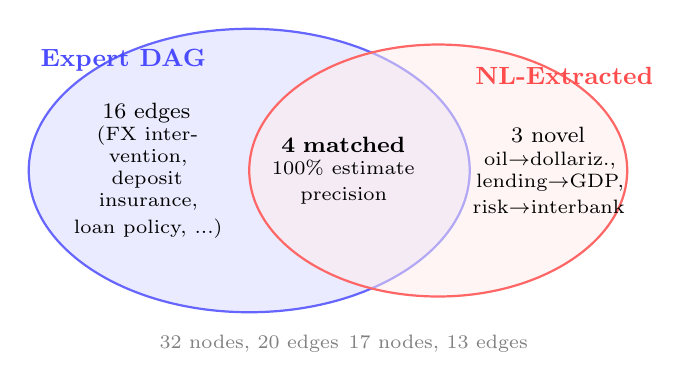
\begin{tikzpicture}[
        every node/.style={font=\small},
    ]
    % Expert circle
    \draw[thick, blue!60, fill=blue!8] (-1.2, 0) ellipse (2.8cm and 1.8cm);
    \node[font=\small\bfseries, blue!70] at (-2.8, 1.4) {Expert DAG};

    % NL circle
    \draw[thick, red!60, fill=red!8, fill opacity=0.5] (1.2, 0) ellipse (2.4cm and 1.6cm);
    \node[font=\small\bfseries, red!70] at (2.8, 1.2) {NL-Extracted};

    % Expert only
    \node[font=\footnotesize, text width=2cm, align=center] at (-2.5, 0) {16 edges\\{\scriptsize (FX intervention,\\deposit insurance,\\loan policy, ...)}};

    % Overlap
    \node[font=\footnotesize, text width=1.8cm, align=center] at (0, 0) {\textbf{4 matched}\\{\scriptsize 100\% estimate\\precision}};

    % NL only
    \node[font=\footnotesize, text width=2.2cm, align=center] at (2.6, 0) {3 novel\\{\scriptsize oil$\to$dollariz.,\\lending$\to$GDP,\\risk$\to$interbank}};

    % Counts
    \node[font=\scriptsize, gray] at (-1.2, -2.2) {32 nodes, 20 edges};
    \node[font=\scriptsize, gray] at (1.2, -2.2) {17 nodes, 13 edges};
    \end{tikzpicture}
    \caption{Comparison of expert-built and NL-extracted DAGs for the Kazakhstan case study. The 4~matched edges achieve 100\% estimate precision. The NL pipeline discovers 3~novel edges with literature support, while missing 16~edges encoding country-specific regulatory details.}
    \label{fig:nl2dag}
\end{figure}

The NL pipeline achieves 20\% structural recall---unsurprising given that a single paragraph cannot encode country-specific regulatory details (central bank FX intervention rules, deposit insurance thresholds, loan classification policy changes). However, all 4~matched edges produce statistically equivalent estimates, and the pipeline discovers 3~novel edges with literature support:

\begin{itemize}[leftmargin=*, itemsep=1pt]
    \item Oil price volatility $\to$ deposit dollarization~\citep{dalgic2024dollarization}
    \item Bank lending standards $\to$ GDP growth (bank lending channel)
    \item Global risk appetite $\to$ domestic interbank rates
\end{itemize}

\subsection{End-to-End Reproducibility}

We run the full agentic pipeline on the KSPI K2 DAG (20~edges) and compare against the expert manual baseline. The pipeline achieves 100\% estimate match (20/20~edges), confirming reproducibility across pipeline modes and adapter dispatch.

\subsection{Issue Detection Effectiveness}

Across 13 pipeline runs on the Kazakhstan case study, the 29-rule engine detects 1{,}479 issues in total, of which 1{,}333 (90.1\%) are \texttt{CRITICAL} severity. PatchBot auto-fixes 812 issues (54.9\%), primarily missing unit specifications (\texttt{UNIT\_MISSING\_IN\_EDGECARD}). Of the 667 remaining open issues, only 19 (1.3\% of total) require human review---demonstrating that the system effectively triages the review burden.

The dominant open issue type is \texttt{SIGNIFICANT\_BUT\_NOT\_IDENTIFIED} (492 instances, 73.8\% of open issues), which fires when an edge achieves $p < 0.05$ but the identifiability screen assigns a claim level below \texttt{IDENTIFIED\_CAUSAL}. This rule alone catches the most common form of overclaiming in applied work. Other frequent detections include \texttt{LOO\_INSTABILITY} (87 instances: leave-one-out sign flips or $>$50\% magnitude changes) and \texttt{RATING\_DIAGNOSTICS\_CONFLICT} (59 instances: A-ratings despite failed diagnostics, auto-downgraded by PatchBot). Figure~\ref{fig:issues} summarizes the issue triage pipeline.

\begin{figure}[t]
    \centering
    \begin{tikzpicture}[
        box/.style={draw, rounded corners=2pt, minimum width=2.2cm, minimum height=0.7cm, font=\scriptsize, align=center},
        arr/.style={-{Stealth[length=4pt]}, thick},
    ]
    % Total
    \node[box, fill=gray!15] (total) at (0, 0) {\textbf{1{,}479 issues}\\detected};
    % Auto-fixed
    \node[box, fill=green!15] (fixed) at (-3.2, -1.5) {\textbf{812 auto-fixed}\\(54.9\%)\\PatchBot};
    % Open
    \node[box, fill=orange!15] (open) at (3.2, -1.5) {\textbf{667 open}\\(45.1\%)};
    % Human review
    \node[box, fill=red!15] (human) at (1.5, -3.0) {\textbf{19 human}\\review (1.3\%)};
    % Automated review
    \node[box, fill=yellow!15] (auto) at (5.0, -3.0) {\textbf{648 flagged}\\for analyst};

    \draw[arr] (total) -- (fixed);
    \draw[arr] (total) -- (open);
    \draw[arr] (open) -- (human);
    \draw[arr] (open) -- (auto);

    % Top issues
    \node[font=\tiny, text width=3cm, align=left, gray, anchor=north west] at (5.0, -0.4) {Top: SIG\_NOT\_ID (492)\\LOO\_INSTAB (87)\\RATING\_CONFLICT (59)};
    \end{tikzpicture}
    \caption{Issue triage across 13 pipeline runs. PatchBot auto-fixes 54.9\% of issues (primarily missing units). Only 1.3\% require human-in-the-loop review, demonstrating effective automation of the governance burden.}
    \label{fig:issues}
\end{figure}

%% ============================================================
%% 10  LIMITATIONS
%% ============================================================
\section{Limitations}
\label{sec:limitations}

\paragraph{NL-to-DAG is lossy.}
Qualifying language is collapsed to binary decisions, effect magnitudes are not reliably extracted from text, and the pipeline cannot distinguish between claims made by the authors and claims they merely cite.

\paragraph{Claims are not identification.}
A DAG extracted from the literature represents \emph{claimed} causal relationships, not identified ones. \oc{}'s identifiability screen partially addresses this, but the initial DAG structure reflects community beliefs rather than proven mechanisms.

\paragraph{Single-country evaluation.}
Our primary case study is Kazakhstan bank stress testing. While the platform is domain-agnostic, the data clients and variable catalogs are currently specific to this use case.

\paragraph{LLM hallucination risk.}
The LLM can fabricate plausible-sounding causal edges not present in the source material. All LLM-extracted edges must be verified against the original text---a requirement that our governance framework enforces via HITL gates but cannot guarantee in fully automated mode.

\paragraph{Independence assumption in propagation.}
The delta-method SE formula (Equation~\ref{eq:delta}) assumes independence across edges. When edges share confounders, standard errors are underestimated. The engine warns but does not correct for this.

%% ============================================================
%% 11  CONCLUSION
%% ============================================================
\section{Conclusion}
\label{sec:conclusion}

\oc{} demonstrates that automation and transparency in causal inference are not mutually exclusive. By treating every modeling decision as an auditable event---logged in a hash-chained ledger, gated by identifiability screens and refutation tests, and protected by anti-p-hacking policies---the platform enables researchers to move faster while maintaining the evidentiary standards that credible causal claims demand. The always-on sentinel loop ensures that this rigor is continuous rather than episodic: the DAG is re-validated after every change, schema regressions are auto-healed, and interactive review panels are surfaced the moment estimation completes. With 18 estimation adapters spanning econometric and ML-based methods, data-driven causal discovery (PC, GES, FCI, NOTEARS), a 4-agent agentic pipeline, and LLM-assisted literature extraction, \oc{} bridges expert-specified and data-driven structure learning within a unified governance framework. We release \oc{} as open-source software to support reproducible causal inference research.

%% ============================================================
%% REFERENCES
%% ============================================================
\bibliographystyle{plainnat}
\bibliography{references}

%% ============================================================
%% APPENDIX
%% ============================================================
\appendix

%% ============================================================
%% APPENDIX A: FULL ISSUE REGISTRY
%% ============================================================
\section{Full Issue Registry}
\label{app:issues}

The \oc{} issue registry contains 29 detection rules organized into six categories. Table~\ref{tab:issue-registry} presents all rules.

\begin{table}[htbp]
\centering
\caption{Full Issue Detection Registry (29 Rules). Trigger: \texttt{pre} = pre-run, \texttt{post} = post-run, \texttt{xrun} = cross-run.}
\label{tab:issue-registry}
\scriptsize
\begin{tabular}{@{}lllllp{4.2cm}@{}}
\toprule
\textbf{Rule ID} & \textbf{Sev.} & \textbf{Scope} & \textbf{Trig.} & \textbf{Fix?} & \textbf{Description} \\
\midrule
\multicolumn{6}{l}{\textit{Data \& Definition}} \\
\texttt{ENTITY\_BOUNDARY\_DRIFT} & HIGH & data & post & No & Mixing entity scopes breaks comparability \\
\texttt{KPI\_DEFN\_MISMATCH} & HIGH & data & xrun & No & NPL/CoR definitions differ across banks \\
\texttt{SHOCK\_CONSTRUCT\_AMBIG} & MED & data & pre & Yes & Missing shock\_node\_id, shock\_unit, shock\_scale \\
\texttt{FREQ\_ALIGNMENT\_ERR} & CRIT & data & pre & Yes & Mixed frequencies without aggregation rule \\
\texttt{FREQ\_SCALING\_MISMATCH} & HIGH & data & xrun & No & Annual vs quarterly not normalized \\
\texttt{EXTRACT\_PROVENANCE\_GAP} & MED & data & post & No & Missing source document/page reference \\
\midrule
\multicolumn{6}{l}{\textit{Identification \& Design}} \\
\texttt{REACTION\_FN\_EDGE} & CRIT & id & pre & No & Reaction edge used for shock propagation \\
\texttt{TIME\_FE\_ABSORBS\_SHOCK} & CRIT & id & pre & Yes & Time FE absorbs common shock; need Exposure$\times$Shock \\
\texttt{EXPOSURE\_NOT\_PREDET} & CRIT & id & pre & No & Exposure variable not pre-treatment \\
\texttt{MECHANICAL\_EDGE\_EST} & HIGH & id & pre & Yes & Accounting identity estimated as regression \\
\texttt{PATH\_DOUBLE\_COUNT} & HIGH & id & post & No & Direct + indirect chain both used \\
\texttt{SIG\_NOT\_IDENTIFIED} & CRIT & id & post & No & $p<0.05$ but claim $\neq$ IDENTIFIED\_CAUSAL \\
\midrule
\multicolumn{6}{l}{\textit{Statistical Inference}} \\
\texttt{SMALL\_SAMPLE\_INF} & HIGH & stat & post & No & $N<30$ with HAC SEs \\
\texttt{PANEL\_FEW\_UNITS} & HIGH & stat & post & No & $<5$ units; cluster-robust unreliable \\
\texttt{LOO\_INSTABILITY} & HIGH & stat & post & No & Leave-one-out sign flip or $>$50\% $\Delta$ \\
\texttt{BREAKS\_UNMODELED} & MED & stat & post & No & Regime changes not in estimation \\
\texttt{MULTI\_TEST\_DRIFT} & MED & stat & xrun & No & Spec search exceeded budget \\
\midrule
\multicolumn{6}{l}{\textit{Time-Series (TSGuard)}} \\
\texttt{NONSTAT\_LEVELS\_RISK} & HIGH & ts & pre & Yes & Both vars trending; need transformation or ECM \\
\texttt{RESID\_AUTOCORR} & MED & ts & post & No & Serial correlation in residuals \\
\texttt{REGIME\_BREAK\_SUSP} & HIGH & ts & post & No & Coefficient instability across splits \\
\texttt{LEADS\_TIMING\_FAIL} & CRIT & ts & post & No & Future shock predicts current outcome \\
\texttt{HAC\_LAG\_SENSITIVE} & MED & ts & post & No & Estimate changes with HAC bandwidth \\
\midrule
\multicolumn{6}{l}{\textit{Selection \& External Validity}} \\
\texttt{SELECT\_PUBLIC\_ONLY} & HIGH & ev & post & No & Only public banks; may not generalize \\
\texttt{SURVIVORSHIP\_BIAS} & HIGH & ev & post & No & Excludes failed/merged banks \\
\texttt{COVERAGE\_GAP\_EV} & MED & ev & post & No & Sample $<$50\% of system assets \\
\midrule
\multicolumn{6}{l}{\textit{Scoring \& Reporting}} \\
\texttt{RATING\_DIAG\_CONFLICT} & HIGH & rpt & post & Yes & A-rating despite failed diagnostics \\
\texttt{N\_REPORT\_INCONSIST} & MED & rpt & post & Yes & Report N $\neq$ EdgeCard N\_eff \\
\texttt{CROSS\_EVID\_CONFLICT} & HIGH & rpt & xrun & No & Same relationship has conflicting signs \\
\texttt{UNIT\_MISSING\_CARD} & CRIT & rpt & post & Yes & EdgeCard missing treatment/outcome unit \\
\bottomrule
\end{tabular}
\end{table}

%% ============================================================
%% APPENDIX B: EDGECARD SCHEMA
%% ============================================================
\section{EdgeCard Schema}
\label{app:edgecard}

The \texttt{EdgeCard} is the primary output artifact---one per estimated edge, both human-readable (YAML) and machine-parseable. It contains the following blocks:

\paragraph{Core identity.} \texttt{edge\_id}, \texttt{dag\_version\_hash} (SHA-256 of DAG at estimation time), \texttt{created\_at}, \texttt{spec\_hash}, \texttt{spec\_details} (design, controls, instruments, FE, SE method).

\paragraph{Estimates.} \texttt{point} ($\hat{\beta}$), \texttt{se}, \texttt{ci\_95}, \texttt{pvalue}, \texttt{treatment\_unit}, \texttt{outcome\_unit}. For local projections: \texttt{horizons}, \texttt{irf}, \texttt{irf\_ci\_lower}, \texttt{irf\_ci\_upper}. Sample sizes: \texttt{n\_calendar\_periods}, \texttt{n\_effective\_obs\_h0}, \texttt{n\_effective\_obs\_by\_horizon}.

\paragraph{Diagnostics.} Dictionary of \texttt{DiagnosticResult} objects, each with: \texttt{name}, \texttt{passed} (bool), \texttt{value} (test statistic), \texttt{threshold}, \texttt{pvalue}, \texttt{message}. Method \texttt{all\_diagnostics\_pass()} returns \texttt{True} if all tests pass.

\paragraph{Identification.} \texttt{claim\_level} $\in$ \{\texttt{IDENTIFIED\_CAUSAL}, \texttt{REDUCED\_FORM}, \texttt{DESCRIPTIVE}, \texttt{BLOCKED\_ID}\}. \texttt{risks} (dict of risk $\to$ severity), \texttt{untestable\_assumptions}, \texttt{testable\_threats\_passed}, \texttt{testable\_threats\_failed}.

\paragraph{Counterfactual block.} \texttt{shock\_scenario\_allowed} (bool), \texttt{policy\_intervention\_allowed} (bool), \texttt{reason\_shock\_blocked}, \texttt{reason\_policy\_blocked}.

\paragraph{Propagation role.} \texttt{role} $\in$ \{\texttt{structural}, \texttt{reduced\_form}, \texttt{bridge}, \texttt{identity}, \texttt{diagnostic\_only}\}. \texttt{mode\_propagation\_allowed} (dict: mode $\to$ bool), \texttt{mode\_shock\_cf\_allowed}, \texttt{mode\_policy\_cf\_allowed}.

\paragraph{Credibility.} \texttt{credibility\_score} (0--1): 40\% diagnostic pass rate + 10\% design strength + 30\% stability + 20\% data coverage. \texttt{credibility\_rating}: A $\geq 0.80$, B $\geq 0.60$, C $\geq 0.40$, D otherwise. Significance is \emph{not} a factor.

\paragraph{Literature.} \texttt{supporting}, \texttt{challenging}, \texttt{methodological} (citation lists), \texttt{search\_status}, \texttt{search\_timestamp}, \texttt{search\_query}, \texttt{total\_results}.

\paragraph{Interpretation boundary.} \texttt{estimand} (what we estimate), \texttt{is\_not} (what this is not), \texttt{channels}, \texttt{population}, \texttt{conditions}, \texttt{allowed\_uses}, \texttt{forbidden\_uses}.

\paragraph{Failure flags.} 8 booleans: \texttt{weak\_identification}, \texttt{potential\_bad\_control}, \texttt{mechanical\_identity\_risk}, \texttt{regime\_break\_detected}, \texttt{small\_sample}, \texttt{high\_missing\_rate}, \texttt{entity\_boundary\_change}, \texttt{definition\_inconsistency}.

%% ============================================================
%% APPENDIX C: QUERY REPL EXAMPLE
%% ============================================================
\section{Query REPL Example Session}
\label{app:repl}

The following annotated session illustrates the \oc{} Query REPL with natural-language query parsing, guardrail enforcement, and hedged narration.

\begin{lstlisting}[basicstyle=\ttfamily\scriptsize, breaklines=true, frame=single]
$ opencausality query --dag config/agentic/dags/kspi_narrative.yaml \
    --mode REDUCED_FORM

  OpenCausality Query REPL
  DAG: Kazakhstan Banking System (23 nodes, 18 edges)
  Cards: 18 | Mode: REDUCED_FORM | Backend: LLM

query> What if oil prices drop 30%?

[Intent classified: shock_scenario]
Source: oil_price | Target: bank_capital_ratio | Magnitude: -0.30

Path 1: oil_price -> income -> bank_capital_ratio
  Edge 1: oil_price_to_income
    Role: reduced_form | Claim: REDUCED_FORM | Coeff: 0.45 | SE: 0.12
    Shock CF: ALLOWED
  Edge 2: income_to_bank_capital_ratio
    Role: structural | Claim: IDENTIFIED_CAUSAL | Coeff: 0.23 | SE: 0.08
    Shock CF: ALLOWED

Guardrail Results:
  [PASS] Mode gating (weakest: REDUCED_FORM, mode allows)
  [PASS] Counterfactual gating (all edges shock-allowed)
  [PASS] TSGuard (no timing failures)
  [PASS] IssueLedger (no CRITICAL issues)
  [PASS] Reaction-function blocking (none in path)
  [PASS] Unit compatibility (pp -> pp)
  [WARN] SE assumes independence (2 estimated edges)

  Effect (per unit):  0.1035
  Scaled (-0.30):    -0.0311
  SE (delta method):  0.0293
  95% CI (scaled):   [-0.089, 0.026]

Narration (hedged):
"In REDUCED_FORM mode, a 30% oil price decline is associated
with a -3.1pp decrease in bank capital ratio (95% CI:
[-8.9pp, +2.6pp]). The first edge (oil -> income) is
REDUCED_FORM; the second is IDENTIFIED_CAUSAL. The effect
is not significant at 5%. SE assumes independence."

query> /mode STRUCTURAL

Mode switched to STRUCTURAL.
WARNING: oil_price_to_income (reduced_form) now BLOCKED.
1 of 2 path edges blocked in STRUCTURAL mode.

query> /quit
\end{lstlisting}

%% ============================================================
%% APPENDIX D: TSGUARD DIAGNOSTICS
%% ============================================================
\section{TSGuard Diagnostic Details}
\label{app:tsguard}

Table~\ref{tab:tsguard-full} details all 7 TSGuard diagnostics with thresholds and governance actions.

\begin{table}[htbp]
\centering
\caption{TSGuard diagnostic tests and governance actions.}
\label{tab:tsguard-full}
\scriptsize
\begin{tabular}{@{}lp{3.5cm}lp{3.5cm}@{}}
\toprule
\textbf{Diagnostic} & \textbf{Description} & \textbf{Threshold} & \textbf{Action on Failure} \\
\midrule
\texttt{leads\_test} & Regress $y_t$ on $x_{t+1}$. Significance $\Rightarrow$ timing failure. & $|\text{corr}| > 0.3$ & \textbf{CRITICAL}: Block CF, cap = BLOCKED\_ID \\
\texttt{residual\_autocorr} & First-order autocorrelation $\rho_1$ of LP residuals. & $|\rho_1| > 0.5$: fail; $> 0.3$: medium & Set autocorr\_risk = high \\
\texttt{hac\_sensitivity} & Re-estimate with NW lags $\{1,4,8\}$. Check sign stability. & Sign flip across bandwidths & Set autocorr\_risk = high \\
\texttt{lag\_sensitivity} & Re-estimate with $L \in \{1,2,4\}$. Check coefficient stability. & Sign flip across lags & Cap rating to B \\
\texttt{regime\_stability} & Split-sample at known breaks (2015-08, 2020-03). & Pre/post sign flip & \textbf{HIGH}: Block CF, cap = REDUCED\_FORM \\
\texttt{placebo\_shift} & Circularly shift treatment by 2--4 periods. & Placebo $p < 0.1$ & Set timing\_risk = high \\
\texttt{shock\_support} & Count episodes $|x_t| > 1\sigma$. & $< 3$ episodes & \textbf{HIGH}: Block CF \\
\bottomrule
\end{tabular}
\end{table}

\paragraph{Dynamics risk categories.} TSGuard assigns 5 risk levels: (1)~\texttt{common\_trend\_risk}---both series persistent ($\text{AC}(1) > 0.9$); (2)~\texttt{autocorr\_risk}---from residual and HAC tests; (3)~\texttt{nonstationarity\_risk}---high AC for both series, cap claim to DESCRIPTIVE unless ECM; (4)~\texttt{regime\_break\_risk}---from split-sample test; (5)~\texttt{timing\_misspec\_risk}---from leads test.

\paragraph{Governance rules.} (1)~Nonstationarity + levels $\Rightarrow$ cap at DESCRIPTIVE; (2)~Lead test failure $\Rightarrow$ BLOCKED\_ID; (3)~Regime instability $\Rightarrow$ cap at REDUCED\_FORM, block CF; (4)~Shock support $< 3$ $\Rightarrow$ block CF. All TSGuard results are stored in EdgeCards and feed into the propagation engine's guardrail~3.

%% ============================================================
%% CODE AVAILABILITY
%% ============================================================
\section*{Code Availability}

\oc{} is open-source software released under the MIT License. The code, DAG specifications, example datasets, and interactive panel outputs are available at:

\begin{center}
\url{https://github.com/LEE-CHENYU/OpenCausality}
\end{center}

\end{document}
